\section{Fourier分解与小波分解的比较}
\label{sec:wavelet-fourier-comparison}

现在可以在同一个空间里比较两种表示。取周期区间$[0,1)$，即空间$L^2(\mathbb T)$。函数在这里还是同一个无限维向量，两组标准正交基给出它的两套坐标。

一套来自第~\ref{chap:fourier-transform}章，换成周期$1$的归一化：$e_n(x)=e^{2\pi\mathrm inx}$（$n\in\mathbb Z$），系数为$\hat f(n)=\langle e_n,f\rangle$。另一套来自定理~\ref{thm:wavelet-periodic-basis}，取周期Haar函数（$j_0=0$），系数为粗项$\int_0^1f$和细节$d_{j,k}=\langle\psi_{j,k},f\rangle$。

两者都给出$L^2$中的正交展开和Parseval等式，区别在于坐标怎样组织：Fourier系数按频率$n$排列，每个$e_n$遍布整个周期；小波系数按尺度$j$和位置$k$排列，每个$\psi_{j,k}$只在长为$2^{-j}$的区间上非零。下面用两个函数检查系数怎样分布，图~\ref{fig:wavelet-coefficient-tiles}汇总了结果。

\begin{BookInlineFigure}
  \centering
  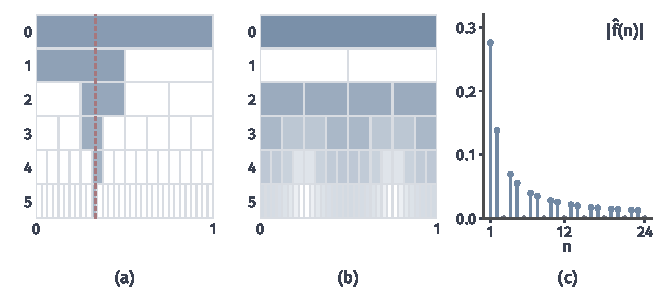
\includegraphics[width=112mm]{figures/04-spaces-measures-and-geometry/03-function-spaces/matplotlib/wavelet-coefficient-tiles/figure.pdf}
  \caption{两种坐标下的系数分布。(a)(b)的每个方格是一个Haar细节系数：纵向为尺度$j$，横向为位置；颜色越深绝对值越大（对数色阶，$10^{-3}$至$1$），白色表示为零。(a)是跳跃函数$\mathbf 1_{[1/3,1)}$，每层只有含跳跃点的一格非零，红色虚线标出$x=1/3$。(b)是$\sin(2\pi x)$，第$1$层全为零，更细的层全部非零。(c)是跳跃函数的Fourier系数绝对值，$n$为$3$的倍数时为零。}
  \label{fig:wavelet-coefficient-tiles}
\end{BookInlineFigure}

\paragraph{平滑振荡}
取$g(x)=\sin(2\pi x)$，$\lVert g\rVert_2^2=1/2$。由$\sin(2\pi x)=(e_1-e_{-1})/(2\mathrm i)$，Fourier系数只有两个非零：
\[
 \hat g(1)=-\frac{\mathrm i}2,\qquad\hat g(-1)=\frac{\mathrm i}2.
\]
两项就精确表示了$g$。

Haar系数则遍布各层。粗项$\int_0^1g=0$。对第$j$层区间$[a,a+h)$，$h=2^{-j}$，记中点$m=a+h/2$，由和差化积，
\begin{equation*}
\begin{aligned}
 \int_a^{m}g-\int_m^{a+h}g
 &=\frac{\cos2\pi a+\cos2\pi(a+h)-2\cos2\pi m}{2\pi}\\
 &=-\frac{2}{\pi}\cos(2\pi m)\sin^2\frac{\pi h}{2}.
\end{aligned}
\end{equation*}
乘以$2^{j/2}$，就得到
\begin{equation}
 d_{j,k}=-\frac{2}{\pi}\,2^{j/2}\cos(2\pi m_{j,k})\sin^2\bigl(\pi2^{-j-1}\bigr).
 \label{eq:wavelet-sine-coefficients}
\end{equation}

逐层读这个公式。$j=0$时$m=1/2$，$d_{0,0}=2/\pi$。$j=1$时两个中点$1/4,3/4$处余弦为零，这一层全为零，因为$g$在每个半周期内关于中点对称。$j\geq2$时中点$(2k+1)2^{-j-1}$都不是$1/4$或$3/4$，这一层的$2^j$个系数全不为零，量级约为$(\pi/2)2^{-3j/2}$，与定理~\ref{thm:wavelet-moment-decay}的Haar估计一致。

\paragraph{局部跳跃}
取$f=\mathbf{1}_{[1/3,1)}$，$\lVert f\rVert_2^2=2/3$。Fourier系数$\hat f(0)=2/3$，$n\neq0$时
\[
 \hat f(n)=\int_{1/3}^1e^{-2\pi\mathrm inx}\,dx=\frac{e^{-2\pi\mathrm in/3}-1}{2\pi\mathrm in}.
\]
取绝对值，得到
\[
 \lvert\hat f(n)\rvert=\frac{\lvert\sin(\pi n/3)\rvert}{\pi\lvert n\rvert}.
\]
$n$是$3$的倍数时为零，其余时为$\sqrt3/(2\pi\lvert n\rvert)$。一处跳跃使无穷多个频率的系数非零，只按$1/\lvert n\rvert$衰减。

Haar系数则高度集中。粗项为$2/3$。若$f$在第$j$层区间上取常值，那里的细节为零，所以每一层只有包含$1/3$的那个区间给出非零系数。沿用第~\ref{sec:wavelet-coefficients-reconstruction}小节的$t_j$：$t_j=1/3$时，$1/3$落在左半，左半减右半的积分是$h/6-h/2=-h/3$；$t_j=2/3$时落在右半，积分是$0-h/3=-h/3$。

于是每层恰有一个非零系数：
\begin{equation}
 d_{j,k}=-2^{j/2}\cdot\frac{h}{3}=-\frac{2^{-j/2}}3.
 \label{eq:wavelet-jump-coefficients}
\end{equation}
能量核对为
\[
 \Bigl(\frac23\Bigr)^2+\sum_{j\geq0}\frac{2^{-j}}9=\frac49+\frac29=\frac23.
\]

\paragraph{有限项的误差}
表~\ref{tab:wavelet-fourier-haar-budget}列出保留部分系数后的平方误差，误差等于被丢弃系数的平方和。Fourier一列保留$\lvert n\rvert\leq N$的项，Haar一列保留粗项与$j<J$的各层，即$P_Jf$。“非零项数”只计实际非零的系数。数值由上面的系数公式求和得到。

\begin{table}[!htb]
\centering
\caption{跳跃函数$f=\mathbf{1}_{[1/3,1)}$与平滑振荡$g=\sin(2\pi x)$在周期区间上的截断平方误差。Fourier保留$\lvert n\rvert\leq N$，Haar保留$V_J$中的全部系数。}
\label{tab:wavelet-fourier-haar-budget}
\begin{tabular}{lccc}
\toprule
表示与截断 & 保留项数 & $f$的非零项数 & $f$的平方误差\\
\midrule
Fourier，$N=4$ & 9 & 7 & 0.0227\\
Fourier，$N=32$ & 65 & 45 & 0.00307\\
Haar，$J=6$ & 64 & 7 & 0.00347\\
\midrule
表示与截断 & 保留项数 & $g$的非零项数 & $g$的平方误差\\
\midrule
Fourier，$N=1$ & 3 & 2 & 0\\
Haar，$J=3$ & 8 & 5 & 0.0252\\
Haar，$J=6$ & 64 & 61 & 0.000401\\
\bottomrule
\end{tabular}
\end{table}

\paragraph{读表}
对跳跃函数，若按固定的项数预算比较，$J=6$的Haar用$64$个位置得到$0.00347$，$N=32$的Fourier用$65$个位置得到$0.00307$，两者相当：线性地截掉高频或细层，误差都大致与项数成反比。

差别出现在“只保留非零系数”时。Haar的$64$个位置中只有$7$个非零，而Fourier要达到同样的误差需要几十个非零项；同样用$7$个非零系数，Haar的误差是$0.00347$，Fourier的误差是$0.0227$。不过，Haar的这一优势要求事先知道跳跃的位置，或者按系数大小自适应地选择保留哪些项。

对平滑振荡，结论反过来：Fourier两项精确表示，Haar在$64$个位置上仍有误差，并且误差每加一层只缩小约四倍，因为Haar只有一个消失矩。换用更光滑、消失矩更多的小波，每层误差下降会更快，但仍不能用有限项精确表示一个正弦。

这说明，正如$\mathbb R^N$中同一个向量在一组基下可能稀疏、在另一组基下可能稠密，函数的稀疏性也不是函数本身的性质，而是函数和基的搭配。哪种表示误差更小，取决于函数（全局振荡还是局部突变）、所用的基以及预算的计法（固定位置还是自适应选取）。这种依赖关系的一般刻画属于第~\ref{chap:function-approximation}章的函数逼近问题。
